\documentclass{beamer}
\usetheme{Madrid}
\usepackage{array}
\setbeamertemplate{caption}[numbered]
\title[CST 309 M4]{MANAGEMENT OF SOFTWARE SYSTEMS}
\subtitle{Module 4}
\author{Rijin IK}
\institute[VJEC]{Assistant Professor\\Department of Computer Science and Engineering\\Vimal Jyothi Engineering College\\Chemperi}
\begin{document}
	\begin{frame}
		\titlepage
	\end{frame}
   \begin{frame}{Outline}
   \tableofcontents
   \end{frame}
\section{Software Project Management}
\begin{frame}{Software Project Management}
\textbf{Software Project Management}
\begin{itemize}
	\item Software project management is an essential part of software engineering.
	\item The \textbf{success criteria} for project management obviously \textbf{vary from project to project}
	\item \textbf{Important goals of Software project management} are
	\begin{itemize}
		\item to deliver the software to the customer at the agreed time; 
		\item to keep overall costs within budget
		\item to deliver software that meets the customer’s expectations;
		\item to maintain a coherent and well-functioning development team.
	\end{itemize}
\end{itemize}
\end{frame}
\begin{frame}{Software Project Management}
	\textbf{Factors influencing the project management:}
	\begin{itemize}
		\item Company size
		\item Software customers
		\item Software size
		\item Software type 
		\item Organizational culture
		\item Software development processes
	\end{itemize}
\end{frame}
\begin{frame}{Software Project Management}
	\textbf{Fundamental project management activities: }
	\begin{itemize}
		\item Project planning
		\item Risk management
		\item People management
		\item Reporting 
		\item Proposal writing
	\end{itemize}
\end{frame}
\begin{frame}{Software Project Management}
	\textbf{Project planning }
	\begin{itemize}
		\item Project managers are responsible for planning, estimating, and 
		scheduling project development and assigning people to tasks.
	\end{itemize}
	\textbf{Risk management}
	\begin{itemize}
		\item Project managers have to assess the risks that may affect a 
		project, monitor these risks, and take action when problems arise.
	\end{itemize}
\textbf{People management}
\begin{itemize}
	\item Project managers are responsible for managing a team of 
	people.
	\item They have to choose people for their team and establish ways of working that lead to effective team performance.
\end{itemize}
\textbf{Reporting}
\begin{itemize}
	\item Project managers are usually responsible for reporting on the progress 
	of a project to customers and to the managers of the company developing the 
	software.
\end{itemize}
\end{frame}
\begin{frame}{Software Project Management}
	\textbf{Proposal writing}
	\begin{itemize}
		\item The first stage in a software project may involve writing a 
		proposal to win a contract to carry out an item of work.
		\item The proposal \textbf{describes the 
			objectives of the project and how it will be carried out.}
		\item It usually \textbf{includes cost and schedule estimates} and \textbf{justifies why the project contract should be awarded to a particular organization or team.}
	\end{itemize}
\end{frame}
\section{Risk Management}
\begin{frame}{Risk Management}
	\textbf{Risk Management}
	\begin{itemize}
		\item Risk management \textbf{involves anticipating risks that might affect the project schedule or the quality} of the software being developed, and then taking \textbf{action to avoid these risks.}
		\item Risks can be categorized according to type of risk (technical, 
		organizational, etc.)
	\end{itemize}
\end{frame}
\begin{frame}{Risk Management}
	\textbf{Classification of risks according to what these risks affect}
	\begin{itemize}
		\item Project risks
		\begin{itemize}
			\item \textbf{affect the project schedule or resources}. An example of a 
			project risk is the loss of an experienced system architect
		\end{itemize}
	\item Product risks
	\begin{itemize}
		\item \textbf{affect the quality or performance }of the software being 
		developed. An example of a product risk is the failure of a purchased 
		component to perform as expected.
	\end{itemize}
\item Business risks
\begin{itemize}
	\item \textbf{affect the organization developing or procuring the 
		software. }For example, a competitor introducing a new product is a 
	business risk.
\end{itemize}
You have to anticipate risks, understand their impact on the project, the product, and the business, and 
take steps to avoid these risks. You may need to draw up contingency plans so that, if the risks do 
occur, you can take immediate recovery action.
	\end{itemize}
\end{frame}
\begin{frame}{Risk Management}
\textbf{Risk Management Process}\\
It involves several stages
\begin{itemize}
	\item \textbf{Risk identification:} You should identify possible project, product, and business risks.
	\item \textbf{Risk analysis:} You should assess the likelihood and consequences of these risks.
	\item \textbf{Risk planning:} You should make plans to address the risk, either by avoiding it or by minimizing its 
	effects on the project.
	\item \textbf{Risk monitoring:} You should regularly assess the risk and your plans for risk mitigation and revise these 
	plans when you learn more about the risk.
\end{itemize}
\end{frame}
\begin{frame}{Risk Management}
	\begin{figure}
	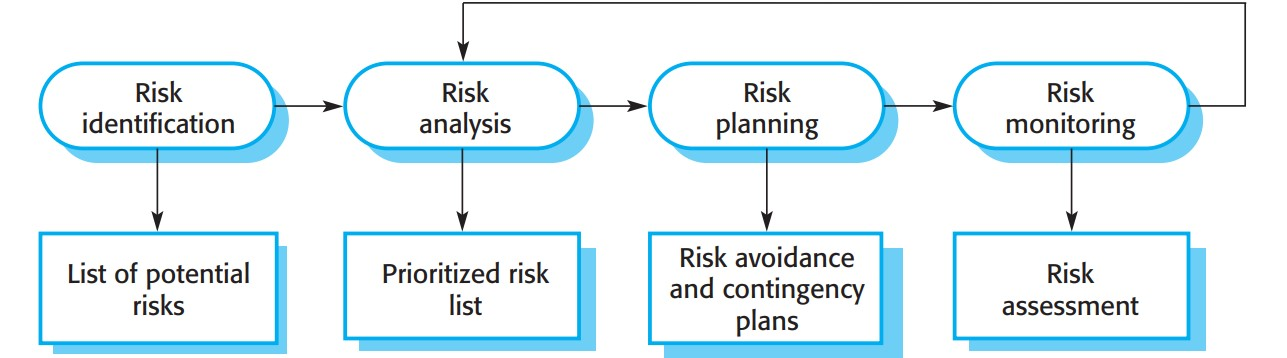
\includegraphics[scale=.45]{img/m4_1}
	\caption{The risk 
		management process
	}
\end{figure}
\end{frame}
\begin{frame}{Risk Management}
\textbf{Risk Identification}
\begin{itemize}
	\item Risk identification is the first stage of the risk management process.
	\item It is concerned with \textbf{identifying the 
		risks that could pose a major threat }to the software engineering process, the software being 
	developed, or the development organization. 
	\item Risk identification \textbf{may be a team process} in which a team gets together to brainstorm possible risks. 
	\item Alternatively, \textbf{project managers may identify risks based on their experience }of what went wrong on 
	previous projects.

	\item  As a starting point for risk identification, a checklist of different types 
	of risk may be used.
\end{itemize}
\end{frame}
\begin{frame}{Risk Management}
	\textbf{Risk Identification cont..}\\6 types of risk may be included in a risk checklist:

	\begin{enumerate}
		\item \textbf{Estimation risks:}arise from the management estimates of the resources 
		required to build the system. 
		\item \textbf{Organizational risks:}arise from the organizational environment where 
		the software is being developed.
		\item \textbf{People risks:}are associated with the people in the development team. 
		\item \textbf{Requirements risks:}come from changes to the customer requirements 
		and the process of managing the requirements change.
		\item \textbf{Technology risks:}come from the software or hardware technologies that 
		are used to develop the system.
		\item \textbf{Tools risks:}come from the software tools and other support software 
		used to develop the system
	\end{enumerate}
\end{frame}
\begin{frame}{Risk Management}
	\textbf{Risk Analysis}
	\begin{itemize}
		\item During the risk analysis process, you have to consider each identified risk and \textbf{make a 
			judgment about the probability and seriousness of that risk. }
		\item It is not possible to make precise, numeric assessment of the probability and seriousness 
		of each risk.

		\item You should assign the risk to one of a number of bands:
		\begin{enumerate}
			\item The probability of the risk might be \textbf{assessed as insignificant, low, moderate, high, or very high. }
			\item The effects of the risk might be assessed as catastrophic (threaten the survival of the project), 
			serious (would cause major delays), tolerable (delays are within allowed contingency), or 
			insignificant.
		\end{enumerate}
	\end{itemize}
\end{frame}
\begin{frame}{Risk Management}
	\textbf{Risk Analysis cont...}
	\begin{itemize}
		\item Once the risks have been analyzed and ranked, you should assess which of these risks are most 
		significant. 
		\item Your judgment must depend on a combination of the probability of the risk arising and the effects of 
		that risk. 
		\item In general, catastrophic risks should always be considered, as should all serious risks that have more 
		than a moderate probability of occurrence.
	\end{itemize}
\end{frame}
\begin{frame}{Risk Management}
	\textbf{Risk Planning}
	\begin{itemize}
		\item The risk planning process\textbf{ develops strategies to manage the key risks 
			that threaten the project.}
		\item For each risk, you have to think of actions that you might take to 
		minimize the disruption to the project if the problem identified in the 
		risk occurs. 
		\item You should also think about the information that you need to collect 
		while monitoring the project so that emerging problems can be 
		detected before they become serious.

		\item In risk planning, you have to ask “what-if” questions that consider both individual risks, combinations of 
		risks, and external factors that affect these risks.

	\end{itemize}
\end{frame}
\begin{frame}{Risk Management}
\textbf{Risk Planning cont...}
\begin{itemize}
	\item Based on the answers to these “what-if” questions, you may devise strategies for managing the risks. 
	These strategies fall into three categories:

	\begin{enumerate}
		\item \textbf{Avoidance strategies:} Following these strategies means that the probability that the risk will arise is 
		reduced. An example of a risk avoidance strategy is the strategy for dealing with defective 
		components
		\item \textbf{Minimization strategies:} Following these strategies means that the impact of the risk is reduced. 
		An example of a risk minimization strategy is the strategy for staff illness
		\item \textbf{Contingency plans:} Following these strategies means that you are prepared for the worst and have 
		a strategy in place to deal with it. An example of a contingency strategy is the strategy for 
		organizational financial problems.
	\end{enumerate}
\end{itemize}
\end{frame}
\begin{frame}{Risk Management}
	\textbf{Risk Monitoring}
	\begin{itemize}
		\item Risk monitoring is the \textbf{process of checking that your assumptions about the product, process, and 
			business risks have not changed. }
		\item You should regularly assess each of the identified risks to decide whether or not that risk is becoming 
		more or less probable. 
	\item You should also think about whether or not the effects of the risk have changed. 
		\item To do this, you have to look at other factors, such as the number of requirements change requests, 
		which give you clues about the risk probability and its effects.
		\item You should monitor risks regularly at all stages in a project. At every management review, you should 
		consider and discuss each of the key risks separately. 
		\item You should decide if the risk is more or less likely to arise and if the seriousness and consequences of 
		the risk have changed.
	\end{itemize}
\end{frame}
\section{Managing people}
\begin{frame}{Managing people}
	\textbf{Managing people}
\begin{itemize}
	\item The people working in a software organization are its greatest assets.
	\item There are \textbf{four critical factors that influence the relationship between a manager and the people that 
		he or she manages:}

	\begin{enumerate}
		\item Consistency:
		\item Respect:
		\item Inclusion:
		\item Honesty: 
	\end{enumerate}
\end{itemize}
\end{frame}
\begin{frame}{Managing people}
%	\textbf{Managing people cont..}
		\begin{enumerate}
			\item \textbf{Consistency:} 
			 All the people in a project team should be treated in a comparable way. No one 
				expects all rewards to be identical, but people should not feel that their contribution to the 
				organization is undervalued.

			
			\item \textbf{Respect:}
				  Different people have different skills, and managers should respect these differences. All 
				members of the team should be given an opportunity to make a contribution.

	
			\item \textbf{Inclusion:}
				 People contribute effectively when they feel that others listen to them and take 
				account of their proposals. It is important to develop a working environment where all views, 
				even those of the least experienced staff, are considered.
			\item \textbf{Honesty: }
			 As a manager, you should always be honest about what is going well and what is going 
				badly in the team. You should also be honest about your level of technical knowledge and be 
				willing to defer to staff with more knowledge when necessary. If you try to cover up ignorance or 
				problems, you will eventually be found out and will lose the respect of the group.
		\end{enumerate}
\end{frame}
\begin{frame}{Managing people}
\textbf{Motivating people:}
\begin{itemize}
	\item As a project manager, you need to motivate the people who work 
	with you so that they will contribute to the best of their abilities. 
	\item In practice, motivation means organizing work and its environment to 
	encourage people to work as effectively as possible.
	\item To provide this encouragement, you should understand a little about 
	what motivates people.
	\item \textbf{People are motivated by satisfying their needs.} These needs are 
	arranged in a series of levels
\end{itemize}
\end{frame}
\begin{frame}{Managing people}

		\begin{figure}
			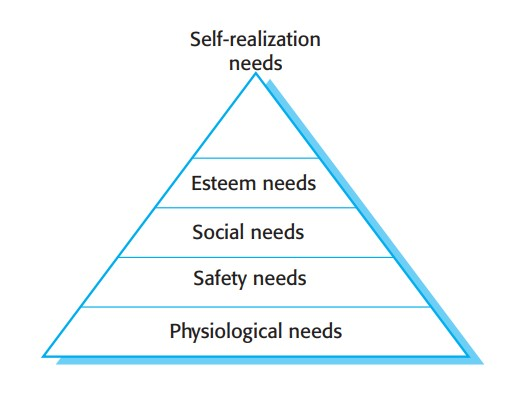
\includegraphics[scale=.45]{img/m4_3}
			\caption{Human 
				needs hierarchy
			}
		\end{figure}
\end{frame}
\begin{frame}{Managing people}
	\textbf{Bass and Dunteman (Bass and Dunteman 1963) identified 3 
		classifications for professional workers:}
	\begin{itemize}
	\item \textbf{Task-oriented people}, who are motivated by the work they do. In software engineering, these are 
	people who are motivated by the intellectual challenge of software development.

	\item \textbf{Self-oriented people,} who are principally motivated by personal success and recognition. They are 
	interested in software development as a means of achieving their own goals. They often have longer term goals, such as career progression, that motivate them, and they wish to be successful in their 
	work to help realize these goals.
	\item \textbf{Interaction-oriented people,} who are motivated by the presence and actions of co-workers. As more 
	and more attention is paid to user interface design, interaction- oriented individuals are becoming 
	more involved in software engineering.

	\end{itemize}
\end{frame}
\section{Teamwork}
\begin{frame}{Teamwork}
\textbf{Teamwork}
\begin{itemize}
	\item Most professional software is developed by \textbf{project teams that range in size from two to several 
		hundred people. }
	\item However, as it is impossible for everyone in a large group to work together on single problem,\textbf{ large 
		teams are usually split into a number of smaller groups. }
	\item\textbf{ Each group is responsible for developing part of the overall system.}
	\item A good group is cohesive and thinks of itself as a strong, single unit. 
	\item The \textbf{people involved are motivated by the success of the group as well as by their own personal goals.}
\end{itemize}
\end{frame}
\begin{frame}{Teamwork}
	\textbf{Teamwork cont..}
	\begin{itemize}
		\item In a \textbf{cohesive group}, members think of the group as more important than the individuals who are group 
		members.
	\begin{itemize}
		\item Members of a well-led, cohesive group are loyal to the group. 
		\item They identify with group goals and other group members. 
		\item They attempt to protect the group, as an entity, from outside interference. 
		\item This makes the group robust and able to cope with problems and unexpected situations.
	\end{itemize}
	\end{itemize}
\end{frame}
\begin{frame}{Teamwork}
	\textbf{Benefits of creating a cohesive group}
	\begin{itemize}
		\item The group can establish its own quality standards. 
		\item Individuals learn from and support each other. 
		\item Knowledge is shared. 
		\item Refactoring and continual improvement is encouraged.
	\end{itemize}
Good project managers should always try to encourage group 
cohesiveness. 
\end{frame}
\begin{frame}{Teamwork}
	Given a stable organizational and project environment,\textbf{ the 3 factors 
		that have the biggest effect on team working are:}
	\begin{itemize}
		\item The people in the group \textbf{(Selecting group members)}
		\item The way the group is organized \textbf{(Group organizations)}
		\item Technical and managerial communications \textbf{(Group communications)}
	\end{itemize}
\end{frame}
\begin{frame}{Teamwork}
\textbf{Selecting team members:}
\begin{itemize}
	\item A manager or team leader’s job is to create a cohesive group and organize that group so that they work 
	together effectively. 
\item This task \textbf{involves selecting a group with the right balance of technical skills and personalities. }
\item Sometimes people are hired from outside the organization; more often, software engineering groups 
	are put together from current employees who have experience on other projects. 
	\item Technical knowledge and ability should not be the only factor used to select group members. 
	\item The “competing engineers” problem can be reduced if the people in the group have complementary 
	motivations. 

\end{itemize}
\end{frame}
\begin{frame}{Teamwork}
	\textbf{Selecting team members cont...}
	\begin{itemize}
	
		\item People who are motivated by the work are likely to be the strongest technically. 
		\item People who are self-oriented will probably be best at pushing the work forward to finish the job. 
		People who are interaction-oriented help facilitate communications within the group
		\item It is sometimes impossible to choose a group with complementary personalities. If this is the case, the 
		project manager has to control the group so that individual goals do not take precedence over 
		organizational and group objectives

	\end{itemize}
\end{frame}
\begin{frame}{Teamwork}
	\textbf{Group Organization}
	\begin{itemize}
		
		\item The way a group is organized affects the group’s decisions, the \textbf{ways 
			information is exchanged, and the interactions between the 
			development group and external project stakeholders. }
		\item Project managers are often responsible for selecting the people in the 
		organization who will join their software engineering team. 
		\item Getting the best possible people in this process is very important as 
		poor selection decisions may be a serious risk to the project. 
		\item Key factors that should influence the selection of staff are education 
		and training, application domain and technology experience, 
		communication ability, adaptability, and problem solving ability.

	\end{itemize}
\end{frame}
\begin{frame}{Teamwork}
	\textbf{Group Communications}
	\begin{itemize}
		\item It is absolutely essential that group members communicate effectively 
		and efficiently with each other and with other project stakeholders. 
		\item Good communication also helps strengthen group cohesiveness.
		\item Group members:

		\begin{itemize}
			\item \textbf{Exchange information} on the status of their work, the design decisions that 
			have been made, and changes to previous design decisions.
			\item\textbf{ Resolve problems} that arise with other stakeholders and inform these 
			stakeholders of changes to the system, the group, and delivery plans. 
			\item \textbf{Come to understand} the motivations, strengths, and weaknesses of other \textbf{people in the group.}
		\end{itemize}
	\end{itemize}
\end{frame}
\begin{frame}{Teamwork}
	\textbf{The effectiveness and efficiency of communications are influenced by:}
	\begin{itemize}
		\item \textbf{Group size:} As a group gets bigger, it gets harder for members to communicate effectively. 
		\item \textbf{Group structure:}People in informally structured groups communicate 
		more effectively than people in groups with a formal, hierarchical structure.
		\item \textbf{Group composition:}People with the same personality may clash, and, as 
		a result, communications can be inhibited.
			\item \textbf{The physical work environment:} The organization of the workplace is a 
				major factor in facilitating or inhibiting communications.
		\item \textbf{The available communication channels:} There are many different forms 
			of communication—face to face, email messages, formal documents, 
			telephone, and technologies such as social networking and wikis.
	\end{itemize}
\end{frame}
\section{Project Planning }
\begin{frame}{Project Planning}
	\textbf{Project Planning}
\begin{itemize}
	\item Project planning is one of the most important jobs of a software project manager. 
	\item As a \textbf{manager,} you \textbf{have to break down the work into parts and assign them to project team members}, anticipate problems that might arise, and prepare tentative solutions to those problems. 
	\item The \textbf{project plan,} which is\textbf{ created at the start of a project and updated as the project progresses,} is used to\textbf{ show how the work will be done} and to assess progress on the project. 
\end{itemize}
\end{frame}
\begin{frame}{Project Planning}
	\textbf{Project Planning}
	\begin{itemize}
		\item Project planning takes place at three stages in a project life cycle
		\begin{itemize}
			\item At the \textbf{proposal stage}, when you are bidding for a contract to develop or provide a software system. You need a plan at this stage to help you decide if you have the resources to complete the work and to work out the price that you should quote to a customer. 
			\item During the \textbf{project startup phase}, when you have to plan who will work on the project, how the project will be broken down into increments, how resources will be allocated across your company, and so on. Here, you have more information than at the proposal stage, and you can therefore refine the initial effort estimates that you have prepared. 
			\item \textbf{Periodically throughout the project}, when you update your plan to reflect new information about the software and its development. You learn more about the system being implemented and the capabilities of your development team. As software requirements change, the work breakdown has to be altered and the schedule extended. 
		\end{itemize}
	\end{itemize}
\end{frame}
\begin{frame}{Project Planning}
	\textbf{Project Planning cont..}
	\begin{itemize}
		\item \textbf{Three main parameters} should be used when \textbf{computing the costs }of a software development project: 
		\begin{itemize}
			\item \textbf{effort costs} (the costs of paying software engineers and managers); 
			\item \textbf{hardware and software costs}, including hardware maintenance and software support; and 
			\item \textbf{travel and training costs}. 
		\end{itemize}
	\item For most projects, the biggest cost is the effort cost. 
	\end{itemize}
\end{frame}
\begin{frame}{Software pricing}
	\textbf{Software pricing}
	\begin{itemize}
		\item In principle, the price of a software system developed for a customer is simply the cost of development plus profit for the developer.
		\item In practice, however, the relationship between the project cost and the price quoted to the customer is not usually so simple.
		\item\textbf{ When calculating a price}, you \textbf{take broader organizational, economic, political, and business considerations into account}(Figure in the next slide).
		\item You need to think about organizational concerns, the risks associated with the project, and the type of contract that will be used.
		\item These issues may cause the price to be adjusted upward or downward
		
	\end{itemize}
\end{frame}
\begin{frame}{Software pricing}
	\begin{figure}
	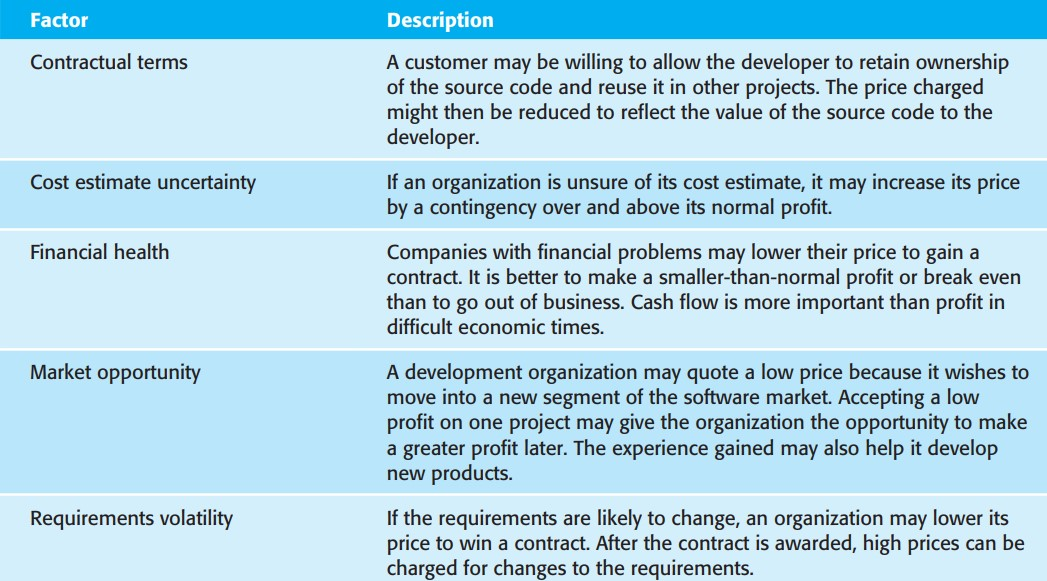
\includegraphics[scale=.5]{img/m4_4}
	\caption{Factors 
		affecting software 
		pricing
	}
\end{figure}
\end{frame}
\begin{frame}{Plan-driven development}
	\textbf{Plan-driven development}
\begin{itemize}
	\item Plan-driven or plan-based development is an approach to software engineering where the 
\textbf{	development process is planned in detail. }
\item A project plan is created that \textbf{records the work to be done, who will do it, the development schedule, 
	and the work products.}
\item Plan-driven development is based on engineering project management techniques and can be thought 
	of as the “traditional” way of managing large software development projects.

\end{itemize}
\end{frame}
\begin{frame}{Plan-driven development}
	\textbf{Plan-driven development cont..}
	\begin{itemize}
		\item Managers \textbf{use the plan to support project decision making} and as a way of \textbf{measuring progress}.
		\item The \textbf{problem with plan-driven development} is that \textbf{early decisions have to be revised} because of 
		changes to the environments in which the software is developed and used. Delaying planning decisions 
		avoids unnecessary rework.
		\item The arguments in favor of a plan-driven approach are that early planning allows organizational issues 
		(availability of staff, other projects, etc.) to be taken into account. Potential problems and 
		dependencies are discovered before the project starts, rather than once the project is underway.
	\end{itemize}
\end{frame}
\begin{frame}{Plan-driven development}
	\textbf{Project Plans}
	\begin{itemize}
		\item In a plan-driven development project, a project plan sets out the resources available to the project, the work breakdown, and a schedule for carrying out the work. 
		
		\item The details of project plans vary depending on the type of project and organization but \textbf{plans normally include the following} sections:
		\begin{itemize}
			\item[1] \textbf{Introduction:} Briefly describes the objectives of the project and sets out the constraints (e.g., budget, time) that affect the management of the project.
			
			\item[2] \textbf{Project organization :}Describes the way in which the development team is organized, the people involved, and their roles in the team.
			\item[3] \textbf{Risk analysis:} Describes possible project risks, and the risk reduction strategies that are proposed.
			\item[4] \textbf{Hardware and software resource requirements:} Specifies the hardware and support software required to carry out the development. If hardware has to be purchased, estimates of the prices and the delivery schedule may be included.
		\end{itemize}
	\end{itemize}
\end{frame}
\begin{frame}{Plan-driven development}
	\textbf{Project Plans cont..}
	\begin{itemize}
	
			\item[5] \textbf{Work breakdown:} Sets out the breakdown of the project into activities and identifies the inputs to and the outputs from each project activity.
			\item[6] \textbf{Project schedule:} Shows the dependencies between activities, the estimated time required to 
			reach each milestone, and the allocation of people to activities. 
			\item[7] \textbf{Monitoring and reporting mechanisms:} Defines the management reports that should be 
			produced, when these should be produced, and the project monitoring mechanisms to be used.
		\end{itemize}

\end{frame}
\begin{frame}{Plan-driven development}
	\textbf{Planning Process}
	\begin{itemize}
		\item Project \textbf{planning is an iterative process} that starts when you create an initial project plan during the project startup phase.
		\item Plan changes are inevitable. As more information about the system and the project team becomes available during the project,\textbf{ you should regularly revise the plan to reflect requirements, schedule, and risk changes}. Changing business goals also leads to changes in project plans. 
	\end{itemize}
\end{frame}
\begin{frame}{Plan-driven development}
	\begin{figure}
	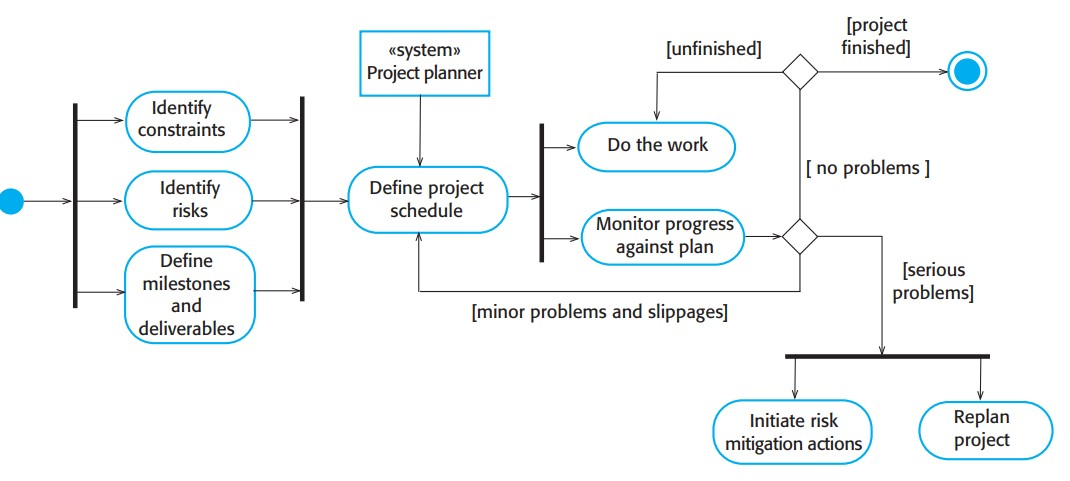
\includegraphics[scale=.5]{img/m4_5}
	\caption{UML activity diagram that shows a typical workflow for a project planning process
	}
\end{figure}
\end{frame}
\begin{frame}{Project Scheduling}
\textbf{Project Scheduling}
\begin{itemize}
	\item Project scheduling is the \textbf{process of deciding how the work in a project will be organized as separate 
		tasks}, and \textbf{when and how these tasks will be executed.}
	\item You\textbf{ estimate the calendar time needed to complete each task} and the effort required, and you suggest 
	who will work on the tasks that have been identified.
	\item You also have to \textbf{estimate the hardware and software resources that are needed to complete each 
		task.}
\end{itemize}
\end{frame}
\begin{frame}{Project Scheduling}
	\textbf{Project Scheduling Activities}
	\begin{itemize}
		\item Scheduling in plan-driven projects involves breaking down the total work involved in a project into 
		separate tasks and estimating the time required to complete each task.
	\end{itemize}
	\begin{figure}
	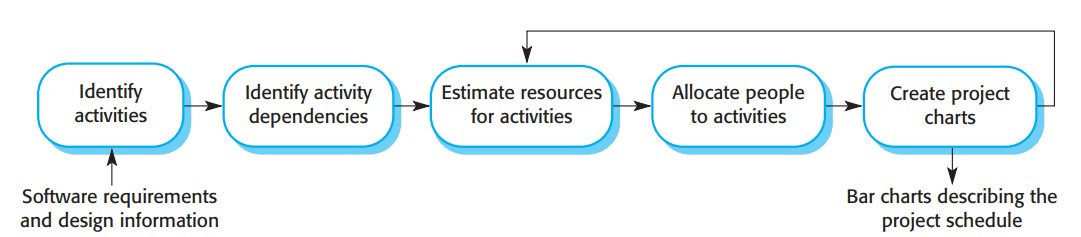
\includegraphics[scale=.5]{img/m4_6}
	\caption{The project 
		scheduling process
	}
\end{figure}
\end{frame}
\begin{frame}{Project Scheduling}
	\textbf{Schedule Presentation}
	\begin{itemize}
		\item Project schedules may simply be documented in a table or spreadsheet showing the tasks, estimated 
		effort, duration, and task dependencies.
		\item \textbf{Two types of visualization} are commonly used:
		\begin{itemize}
			\item \textbf{Calendar-based bar charts} show who is responsible for each activity, the expected elapsed time, 
			and when the activity is scheduled to begin and end. Bar charts are also called Gantt charts, 
			after their inventor, Henry Gantt
			\item \textbf{Activity networks} show the dependencies between the different activities making up a project. 
			These networks are described in an associated web section.
		\end{itemize}
	\end{itemize}
\end{frame}
\begin{frame}{Project Scheduling}
	\textbf{Schedule Presentation cont..}
	\begin{itemize}
		\item \textbf{Project activities} are the basic planning element. \textbf{Each activity has:}
		\begin{itemize}
			\item A \textbf{duration in calendar days} or months
			\item An \textbf{effort estimate}, which shows the number of person-days or person-months to complete the 
			work;
			\item A \textbf{deadline} by which the activity should be complete; and
			\item A \textbf{defined endpoint}, which might be a document, the holding of a review meeting, the 
			successful execution of all tests, or the like
		\end{itemize}
	\end{itemize}
\end{frame}
\begin{frame}{Project Scheduling}
	\textbf{Milestones and deliverables: }
	\begin{itemize}
		\item Milestone is a \textbf{logical end to a stage of the project where the progress of the work can be reviewed}. 
		Each milestone should be documented by a brief report (often simply an email) that summarizes the 
		work done and whether or not the work has been completed as planned. Milestones may be 
		associated with a single task or with groups of related activities.
		\item Some activities create project deliverables—\textbf{outputs that are delivered to the software customer. }
		Usually, the deliverables that are required are specified in the project contract, and the customer’s 
		view of the project’s progress depends on these deliverables. Milestones and deliverables are not the 
		same thing. Milestones are short reports that are used for progress reporting, whereas deliverables are 
		more substantial project outputs such as a requirements document or the initial implementation of a 
		system.
	\end{itemize}
\end{frame}
\begin{frame}{Agile planning}
\textbf{Agile planning}
\begin{itemize}
	\item Agile methods of software development are \textbf{iterative approaches where the software is developed and 
		delivered to customers in increments.}
	\item Unlike plan-driven approaches, the functionality of these increments is not planned in advance but is 
	decided during the development
	\item The decision on what to include in an increment depends on progress and on the customer’s priorities. 
	\item Agile development methods such as Scrum  and Extreme Programming  have a \textbf{two-stage approach to planning}, corresponding to the startup phase in plan-driven development and development planning:
	\begin{enumerate}
		\item \textbf{Release planning,} which looks ahead for several months and decides on the features that should be included in a release of a system.
			\item \textbf{Iteration planning,} which has a shorter term outlook and focuses on planning the next increment of a system. This usually represents 2 to 4 weeks of work for the team.
	\end{enumerate}
\end{itemize}
\end{frame}
\begin{frame}{Agile planning}
	\textbf{Approaches}
	\begin{enumerate}
		\item Planning in Scrum
		
		\item \textbf{Planning game:} developed as part of Extreme Programming, is based on user stories. The so-called 
		planning game can be used in both release planning and iteration planning.
	\end{enumerate}
\end{frame}
\begin{frame}{Agile planning}
	\begin{figure}
	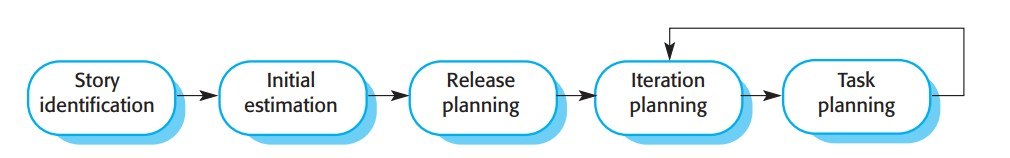
\includegraphics[scale=.5]{img/m4_7}
	\caption{The “planning game”}
\end{figure}
\end{frame}
\begin{frame}{Agile planning}
	\textbf{Agile planning}
	\begin{enumerate}
		\item Story Based Planning
		\item Task Allocation
	\end{enumerate}
\end{frame}
\begin{frame}{Agile planning}
\textbf{Story Based Planning:}
\begin{itemize}
	\item The basis of the planning game is a set of user stories that cover all of the functionality to be included 
	in the final system.
	\item The team members read and discuss the stories and rank them based on the amount of time they think 
	it will take to implement the story
\end{itemize}
\textbf{Task Allocation}
\begin{itemize}
	\item During task planning stage where the developers break down stories into development tasks.
	\item A development task should take 4–16 hours. 
	\item All of the tasks that must be completed to implement all of the stories in that iteration are listed. 
	\item The individual developers then sign up for the specific tasks that they will implement.
\end{itemize}
\end{frame}
\begin{frame}{Agile planning}
\textbf{Agile Planning Difficulties}
\begin{itemize}
	\item A major difficulty in agile planning is that it relies on\textbf{ customer involvement and availability. }
	\item This involvement can be \textbf{difficult to arrange, as customer representatives} sometimes have to prioritize 
	other work and are not available for the planning game.
	\item Furthermore, some \textbf{customers may be more familiar with traditional project plans and may find it 
		difficult to engage in an agile planning process.}
\end{itemize}
\end{frame}
\begin{frame}{Agile planning}
	\textbf{Agile Planning Applicability:}
	\begin{itemize}
		\item Agile planning works well with small, stable development teams that can get 
		together and discuss the stories to be implemented.
		\item However, where teams are large and/or geographically distributed, or when team membership 
		changes frequently, it is practically impossible for everyone to be involved in the collaborative planning 
		that is essential for agile project management.
		
	\end{itemize}
\end{frame}
\section{Estimation Techniques}
\begin{frame}{Estimation Techniques}
\textbf{Estimation Techniques}\\Two types of techniques can be used for making estimates:
\begin{enumerate}
	\item \textbf{Experience-based techniques:}
	\begin{itemize}
		\item The estimate of future effort requirements is\textbf{ based on the manager’s 
			experience of past projects and the application domain}. Essentially, the manager makes an informed 
		judgment of what the effort requirements are likely to be.

	\end{itemize}
	\item \textbf{Algorithmic cost modeling:}
	\begin{itemize}
		\item In this approach, a\textbf{ formulaic approach is used} to compute the project 
		effort \textbf{based on estimates of product attributes,} such as \textbf{size, process characteristics, and experience 
			of staff involved.}
	\end{itemize}
\end{enumerate}
\end{frame}
\begin{frame}{Estimation Techniques}
\textbf{Experience based techniques:}
\begin{itemize}
	\item Experience-based techniques \textbf{rely on the manager’s experience of past projects and the actual effort 
		expended in these projects} on activities that are related to software development.
	\item Typically, you identify the deliverables to be produced in a project and the different software 
	components or systems that are to be developed. 
\item You document these in a spreadsheet, estimate them individually, and compute the total effort 
	required. 
\item It usually helps to get a group of people involved in the effort estimation and to ask each member of 
	the group to explain their estimate.
\end{itemize}
\end{frame}
\begin{frame}{Estimation Techniques}
	\textbf{Experience based techniques cont...}
	\begin{itemize}
		\item The difficulty with experience-based techniques is that a new software project may not have much in 
		common with previous projects. 
		\item Software development changes very quickly, and a project will often 
		use unfamiliar techniques such as web services, application system configuration, or HTML5.
		\item If you 
		have not worked with these techniques, your previous experience may not help you to estimate the 
		effort required, making it more difficult to produce accurate costs and schedule estimates
	\end{itemize}
\end{frame}
\begin{frame}{Estimation Techniques}
	\textbf{Algorithmic cost Modeling:}
	\begin{itemize}
		\item Algorithmic cost modeling \textbf{uses a mathematical formula to predict} project costs based on estimates of 
		the project size, the type of software being developed, and other team, process, and product factors.

		\item Most algorithmic models for estimating effort in a software project are based on a simple formula:
		\begin{center}
			$Effort\  = A * SizeB * M$
		\end{center}
		\begin{itemize}
			\item \textbf{ A:} a constant factor, which depends on local organizational practices and the type of software that 
			is developed.
			\item \textbf{Size:} an assessment of the code size of the software or a functionality estimate expressed in 
			function or application points.

			\item \textbf{B:} represents the complexity of the software and usually lies between 1 and 1.5.
			\item \textbf{M:} is a factor that takes into account process, product and development attributes, such as the 
			dependability requirements for the software and the experience of the development team.
		\end{itemize}
	\end{itemize}
\end{frame}
\begin{frame}{Estimation Techniques}
	\textbf{Algorithmic cost Modeling cont..}
	\begin{itemize}
		\item The idea of using a scientific and objective approach to cost estimation is an attractive one, but all 
		algorithmic cost models suffer from two key problems:
		\begin{itemize}
			\item Algorithmic cost models are a systematic way to estimate the effort required to develop a system. 
			However, these models are complex and difficult to use. 
			\item There are many attributes and considerable scope for uncertainty in estimating their values. 
		\item This complexity means that the practical application of algorithmic cost modeling has been limited to a 
			relatively small number of large companies, mostly working in defense and aerospace systems 
			engineering.
		\item Another barrier that discourages the use of algorithmic models is the need for calibration. Model users 
			should calibrate their model and the attribute values using their own historical project data, as this 
			reflects local practice and experience.
		\end{itemize}
	\end{itemize}
\end{frame}
\begin{frame}{Estimation Techniques}
	\textbf{Effectiveness of this Model:}
	\begin{itemize}
		\item Algorithmic cost models are a systematic way to estimate the effort required to develop a system. 
		However, \textbf{these models are complex and difficult to use.} 
		\item There are many attributes and considerable scope for uncertainty in estimating their values. 
		\item This complexity means that the practical application of algorithmic cost modeling has been limited to a 
		relatively small number of large companies, mostly working in defense and aerospace systems 
		engineering.
		\item Another barrier that discourages the use of algorithmic models is the need for calibration. Model users 
		should calibrate their model and the attribute values using their own historical project data, as this 
		reflects local practice and experience.
	
	\end{itemize}
\end{frame}
\begin{frame}{COCOMO cost modeling. }
\textbf{COCOMO cost modeling.}
\begin{itemize}
	\item The Constructive Cost Model\textbf{(COCOMO) is a procedural software cost estimation model} developed by Barry W Boehm
	\item COCOMO Model is\textbf{ used to estimate size, cost and time of software to be developed}
	\item The best known algorithmic cost modeling technique and tool is the COCOMO II
	\item The submodels that are part of the COCOMO II model are:
	\begin{enumerate}
		\item The application composition model
		\item The early design model
		\item The reuse model
		\item The post-architecture level

	\end{enumerate}
\end{itemize}
\end{frame}
\begin{frame}{COCOMO cost modeling. }
		\begin{figure}
			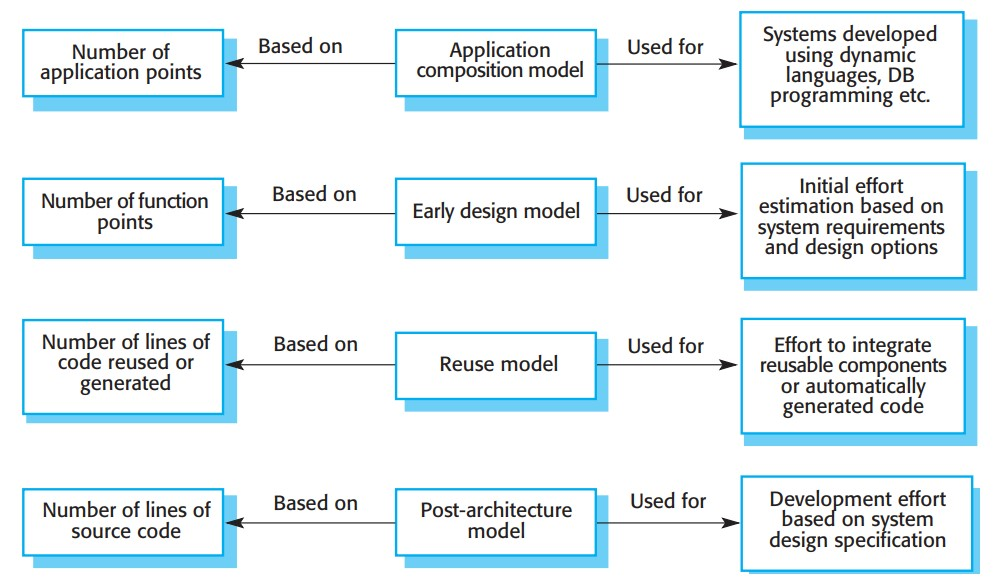
\includegraphics[scale=.5]{img/m4_8}
			\caption{COCOMO 
				estimation models
			}
		\end{figure}
\end{frame}
\begin{frame}{COCOMO cost modeling. }
\textbf{An application composition model}
\begin{itemize}
	\item This models \textbf{the effort required to develop 
		systems that are created from reusable components, scripting, or database programming.}
	\item \textbf{Software size estimates are based on application points}, and a simple size/productivity formula is used to estimate the effort required.
	\item Formula is
	 $$ PM = (NAP * (1 - \%reuse/100)) / PROD $$
	 \textbf{PM} is the effort in person-months,\\
	 \textbf{NAP} is the number of application points and\\
	 \textbf{PROD} is the productivity.
\end{itemize}
\end{frame}
\begin{frame}{COCOMO cost modeling. }
	\textbf{Early design model}
	\begin{itemize}
		\item  This model is \textbf{used during early stages of the system 
			design after the requirements have been established}. 
		\item The \textbf{estimate is based on the 
			standard estimation formula} with a simplified set of seven multipliers. Estimates are based on function points, 
		which are then converted to number of lines of source code.
	\end{itemize}
\end{frame}
\begin{frame}{COCOMO cost modeling. }
	\textbf{Early design model cont...}
	\begin{itemize}
		\item  Based on a standard formula for algorithmic models
		$$ PM = 2.94 * Size(1.1 to 1.24) * M $$
		$$ Where\  M = PERS * PREX * RCPX * RUSE * PDIF * SCED * FSIL $$
		\textbf{2.94} is initial calibration,\\
		\textbf{PERS:} personnel capability,\\
		\textbf{PREX:} personnel experience,\\
		\textbf{RCPX:} product reliability and complexity\\
		\textbf{RUSE:} reuse required\\
		\textbf{PDIF:} platform difficulty\\
		\textbf{SCED:} schedule\\
		\textbf{FSIL:} support facilities\\
		Size in KLOC(The size of the code for the project in Kilo lines of code)\\
	\end{itemize}
\end{frame}
\begin{frame}{COCOMO cost modeling. }
	\textbf{The reuse model}
	\begin{itemize}
		\item  This model is \textbf{used to compute the effort required to integrate 
			reusable components and/or automatically generated program code.}
		\item It is normally used in conjunction with the post-architecture model.
		\item There are two versions:
		\begin{enumerate}
			\item Black-box reuse where code is not modified. An effort estimate (PM) is computed.
			\item White-box reuse where code is modified. A size estimate equivalent to the number
			of lines of new source code is computed. This then adjusts the size estimate for new
			code.
		\end{enumerate}
	\end{itemize}
\end{frame}
\begin{frame}{COCOMO cost modeling. }
	\textbf{The reuse model}
	\begin{itemize}
		\item  Reuse model estimates 1:
		\begin{itemize}
			\item For generated code $$ PM = (ASLOC * AT/100)/ATPROD $$
		\textbf{ASLOC} is the number of lines of generated code\\
			\textbf{AT} is the percentage of code automatically generated.\\
			\textbf{ATPROD} is the productivity of engineers in integrating this code\\
		\end{itemize}
	\item Reuse model estimates 2:
	\begin{itemize}
		\item When code has to be understood and integrated:$$ESLOC = ASLOC * (1-AT/100) * AAM.$$
		\item ASLOC and AT as before.
		\item \textbf{AAM } is the adaptation adjustment multiplier computed from the costs of
		changing the reused code, the costs of understanding how to integrate the code
		and the costs of reuse decision making.
	\end{itemize}
	\end{itemize}
\end{frame}
\begin{frame}{COCOMO cost modeling. }
	\textbf{A post-architecture model}
	\begin{itemize}
		\item Once the system architecture has been designed, a 
		more accurate estimate of the software size can be made. 
		\item Again, this model uses 
		the standard formula for cost estimation discussed above. 
		\item However, it includes 
		a more extensive set of 17 multipliers reflecting personnel capability, product, 
		and project characteristics.
	\end{itemize}
\end{frame}
\section{Configuration Management}
\begin{frame}{Configuration Management}
	\textbf{Configuration Management}
	\begin{itemize}
		\item Configuration management (CM) is concerned with the policies, processes, and tools for managing changing software systems.
		\item The configuration management of a software system product involves four closely related activities:
		\begin{enumerate}
			\item \textbf{Version control:} This involves keeping track of the multiple versions of system components and 
			ensuring that changes made to components by different developers do not interfere with each other.

			\item \textbf{System building:} This is the process of assembling program components, data, and libraries, then 
			compiling and linking these to create an executable system.
			\item \textbf{Change management:} This involves keeping track of requests for changes to delivered software from 
			customers and developers, working out the costs and impact of making these changes, and deciding if 
			and when the changes should be implemented.
			\item \textbf{Release management:} This involves preparing software for external release and keeping track of the 
			system versions that have been released for customer use.
		\end{enumerate}
	\end{itemize}
\end{frame}
\begin{frame}{Configuration Management}
	\begin{figure}
	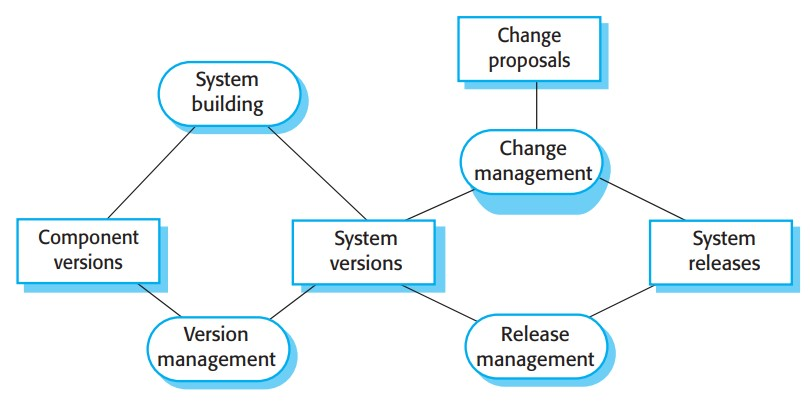
\includegraphics[scale=.5]{img/m4_9}
	\caption{Configuration 
		management activities}
\end{figure}
\end{frame}
\begin{frame}{Configuration Management}
\textbf{Configuration Management cont..}
\begin{itemize}
	\item The development of a software product or custom software system takes place in three distinct phases:
	\begin{itemize}
		\item  A\textbf{ development phase} where the development team is responsible for managing the software 
		configuration and new functionality is being added to the software. The development team decides on 
		the changes to be made to the system.
		\item A \textbf{system testing phase }where a version of the system is released internally for testing. This may be the 
		responsibility of a quality management team or an individual or group within the development team. 
		At this stage, no new functionality is added to the system. The changes made at this stage are bug fixes, 
		performance improvements, and security vulnerability repairs. There may be some customer 
		involvement as beta testers during this phase.
		\item A \textbf{release phase} where the software is released to customers for use. After the release has been 
		distributed, customers may submit bug reports and change requests. New versions of the released 
		system may be developed to repair bugs and vulnerabilities and to include new features suggested by 
		customers.
	\end{itemize}
\end{itemize}
\end{frame}
\begin{frame}{Configuration Management}
\textbf{Multi – version system}
\begin{itemize}
	\item For large systems, there is never just one “working” version of a system; there are always several versions 
	of the system at different stages of development. Several teams may be involved in the development of 
	different system versions.
\end{itemize}

	\begin{figure}
	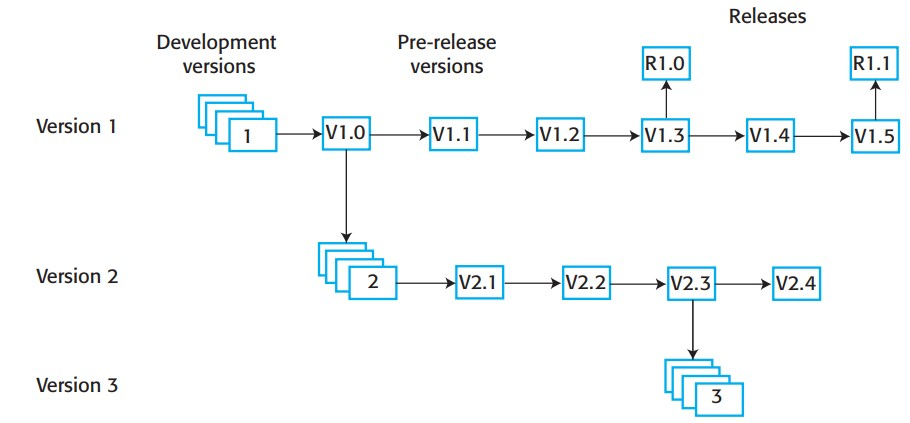
\includegraphics[scale=.5]{img/m4_10}
	\caption{Multiversion system 
		development}
\end{figure}
\end{frame}
\begin{frame}{Configuration Management}
	\begin{figure}
	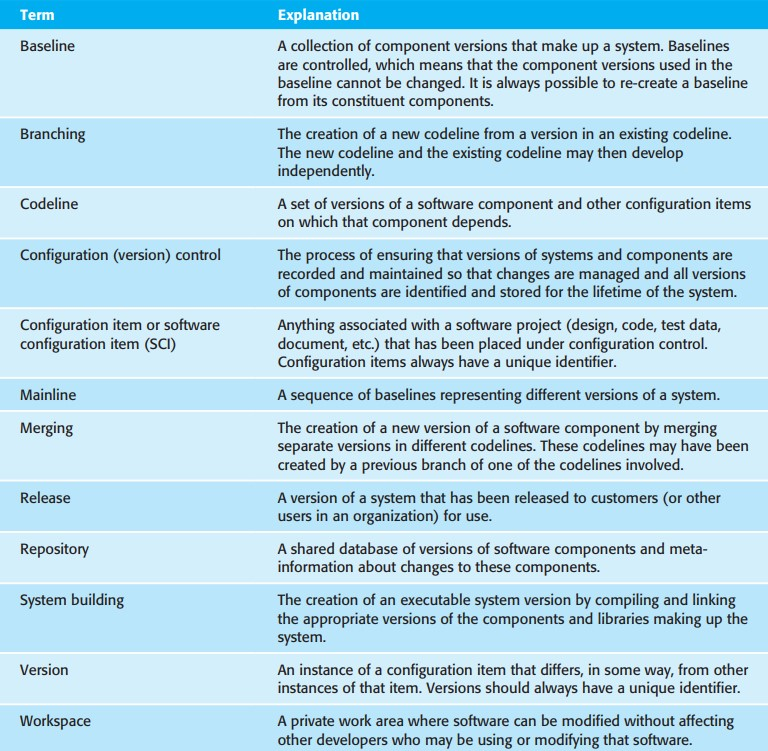
\includegraphics[scale=.5]{img/m4_11}
	\caption{CM 
		terminology}
\end{figure}
\end{frame}
\begin{frame}{Configuration Management}
\textbf{Version Management}
\begin{itemize}
	\item Version management is the process of keeping track of different versions of software components and 
	the systems in which these components are used.
	\item It also involves ensuring that changes made by 
	different developers to these versions do not interfere with each other. \item In other words, version 
	management is the process of \textbf{managing code lines and baselines.}
\end{itemize}
\end{frame}
\begin{frame}{Configuration Management}
	\textbf{Version Management cont..}
	\begin{itemize}
		\item A \textbf{codeline} is a sequence of versions of source code, with later versions in the sequence derived from 
		earlier versions. Code lines normally apply to components of systems so that there are different 
		versions of each component. 
		\item A \textbf{baseline} is a definition of a specific system. The baseline specifies the component versions that are 
		included in the system and identifies the libraries used, configuration files, and other system 
		information

	\end{itemize}
\end{frame}
\begin{frame}{Version Management}
	\textbf{Version Control Systems}
	\begin{itemize}
		\item Version control (VC) systems identify, store, and control access to the different versions of components.
		\begin{itemize}
			\item There are two types of modern version control system:
			\begin{enumerate}
				\item  \textbf{Centralized systems}, where a single master repository maintains all versions of the software 
				components that are being developed. Subversion is a widely used example of a centralized VC system.
				\item \textbf{Distributed systems}, where multiple versions of the component repository exist at the same time. Git is 
				a widely used example of a distributed VC system
			\end{enumerate}
		\end{itemize}
	\end{itemize}
\end{frame}
\begin{frame}{Version Management}
	\textbf{Key features of Version Control Systems}
	\begin{itemize}
		\item Version and release identification
		\item Change history recording
		\item Independent development
		\item Project support
		\item Storage management
		\end{itemize}
\end{frame}
\begin{frame}{Configuration Management}
	\textbf{System Building}
	\begin{itemize}
		\item System building is the process of creating a complete, executable system by compiling and linking the 
		system components, external libraries, configuration files, and other information.
	\item System building involves assembling a large amount of information about the software and its 
		operating environment.

	\end{itemize}
\begin{figure}
	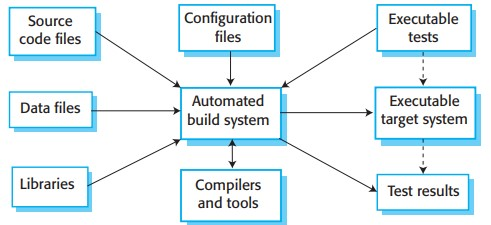
\includegraphics[scale=.5]{img/m4_12}
	\caption{System Building}
\end{figure}
\end{frame}
\begin{frame}{System Building}
	\textbf{System Building functionality}
	\begin{itemize}
		\item \textbf{Build script generation:} The build system should analyze the program that is being built, identify 
		dependent components, and automatically generate a build script (configuration file).
		\item \textbf{Version control system integration:} The build system should check out the required versions of 
		components from the version control system.
		\item \textbf{Minimal recompilation:} The build system should work out what source code needs to be recompiled 
		and set up compilations if required.
		\item \textbf{Executable system creation:} The build system should link the compiled object code files with each 
		other and with other required files, such as libraries and configuration files, to create an executable 
		system.
	\end{itemize}
\end{frame}
\begin{frame}{System Building}
	\textbf{System Building functionality cont...}
	\begin{itemize}
		\item \textbf{Test automation:} Some build systems can automatically run automated tests using test automation 
		tools such as JUnit. These check that the build has not been “broken” by changes.
		\item \textbf{Reporting:} The build system should provide reports about the success or failure of the build and the 
		tests that have been run.
		\item \textbf{Documentation generation:} The build system may be able to generate release notes about the build 
		and system help pages.
	\end{itemize}
\end{frame}
\begin{frame}{System Building}
	\textbf{System Platforms:}
	\begin{itemize}
		\item The development system, which includes development tools such as compilers and source code editors.
	\item \textbf{The build server:} This is used to build definitive, executable versions of the system. This server 
		maintains the definitive versions of a system.
		\item \textbf{The target environment,} which is the platform on which the system executes. This may be the same 
		type of computer that is used for the development and build systems.
	\end{itemize}
\end{frame}
\begin{frame}{System Building}
	\textbf{Continuous Integration}\\
	Steps in Continuous Integration:
	\begin{itemize}
		\item Extract the mainline system from the VC system into the developer’s private workspace.
		\item Build the system and run automated tests to ensure that the built system passes all tests
		\item Make the changes to the system components.
		\item Build the system in a private workspace and rerun system tests. If the tests fail, continue editing
		\item Once the system has passed its tests, check it into the build system server but do not commit it as a 
		new system baseline in the VC system.
		\item Build the system on the build server and run the tests
		\item If the system passes its tests on the build system, then commit the changes you have made as a new 
		baseline in the system mainline.
	\end{itemize}
\end{frame}
\begin{frame}{System Building}
	\textbf{Continuous Integration cont..}\\
%	Steps in Continuous Integration:
	\begin{itemize}
		\item The advantage of continuous integration is that it allows problems caused by the interactions between 
		different developers to be discovered and repaired as soon as possible.
		\item If the system is very large, it may take a long time to build and test, especially if integration with other 
		application systems is involved.
		\item If the development platform is different from the target platform, it may not be possible to run system 
		tests in the developer’s private workspace.
	\end{itemize}
\end{frame}
\begin{frame}{Configuration Management}
	\textbf{Change Management:}
	\begin{itemize}
		\item Organizational needs and requirements change during the lifetime of a system, bugs have to be 
		repaired, and systems have to adapt to changes in their environment.
		\item Change management is intended to ensure that the evolution of the system is controlled and that the 
		most urgent and cost-effective changes are prioritized.
		\item Change management is the process of analyzing the costs and benefits of proposed changes, approving 
		those changes that are cost-effective, and tracking which components in the system have been 
		changed

	\end{itemize}
\end{frame}
\begin{frame}{Change Management}
	\textbf{Factors in change analysis:}
	\begin{itemize}
		\item \textbf{The consequences of not making the change:} When assessing a change request, you have to consider 
		what will happen if the change is not implemented. If the change is associated with a reported system 
		failure, the seriousness of that failure has to be taken into account
		\item \textbf{The benefits of the change:} Will the change benefit many users of the system, or will it only benefit the 
		change proposer?
		\item \textbf{The number of users affected by the change:} If only a few users are affected, then the change may be 
		assigned a low priority.
		\item \textbf{The costs of making the change:} If making the change affects many system components and/or takes a 
		lot of time to implement, then the change may be rejected
		\item \textbf{The product release cycle:} If a new version of the software has just been released to customers, it may 
		make sense to delay implementation of the change until the next planned release.

	\end{itemize}
\end{frame}
\begin{frame}{Configuration Management}
	\textbf{Release Management:}
	\begin{itemize}
		\item A system release is a version of a software system that is distributed to customers.
		\item  For mass-market 
		software, it is usually possible to identify two types of release: major releases, which deliver significant 
		new functionality, and minor releases, which repair bugs and fix customer problems that have been 
		reported.
	\end{itemize}
\end{frame}
\begin{frame}{Release Management}
	\textbf{Release components:}
	\begin{itemize}
		\item A software product release is not just the executable code of the system.
		\item The release may also include:
		\begin{itemize}
			\item configuration files defining how the release should be configured for particular installations;
			\item data files, such as files of error messages in different languages, that are needed successful system 
			operation;
			\item an installation program that is used to help install the system on target hardware;
		\item electronic and paper documentation describing the system;
			\item packaging and associated publicity that have been designed for that release.
		\end{itemize}
	\end{itemize}
\end{frame}
\begin{frame}{Release Management}
	\begin{figure}
		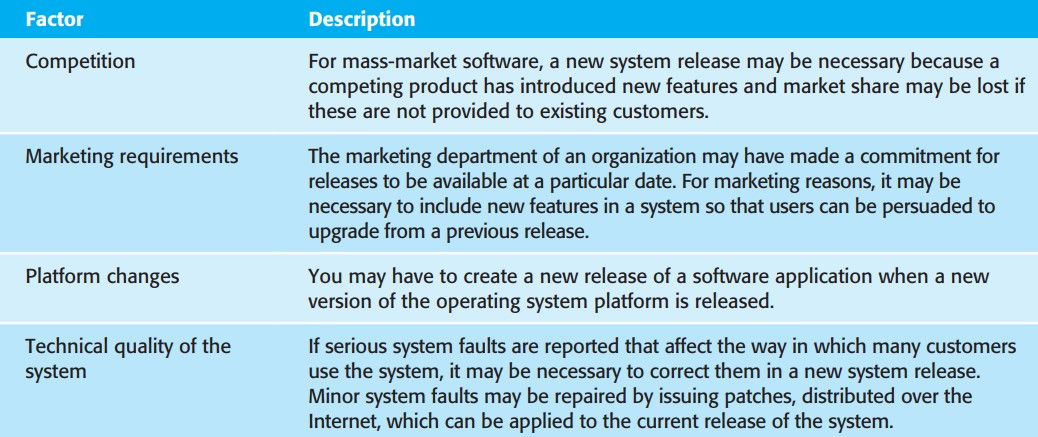
\includegraphics[scale=.5]{img/m4_13}
		\caption{Factors 
			influencing system 
			release planning}
	\end{figure}
\end{frame}
\begin{frame}{Release Management}
	\begin{itemize}
		\item Release creation is the process of creating the collection of files and documentation that include all 
		components of the system release.
		\item This process involves several steps
		\begin{enumerate}
			\item The executable code of the programs and all associated data files must be identified in the version 
			control system and tagged with the release identifier.
			\item Configuration descriptions may have to be written for different hardware and operating systems.
			\item Updated instructions may have to be written for customers who need to configure their own 
			systems.
			\item Scripts for the installation program may have to be written.
			\item Web pages have to be created describing the release, with links to system documentation.
			\item Finally, when all information is available, an executable master image of the software must be 
			prepared and handed over for distribution to customers or sales outlets.
		\end{enumerate}
	\end{itemize}
\end{frame}
\section{SCRUM FRAMEWORK}
\begin{frame}{SCRUM FRAMEWORK}
\textbf{SCRUM FRAMEWORK}
\begin{itemize}
	\item Scrum is an agile software development. 
	\item Scrum principles are consistent with agile manifesto and are used to guide development activities 
	within a process that incorporates the following framework actives: requirements, analysis, design, 
	evolution and delivery.
	\item Within each process activities task work within a process pattern called sprint. 
	\item The work conducted within a sprint is adapted to the problem at hand and is defined and often 
	modified by the Scrum team.
	\item Scrums emphasize the use of set of software patterns that have been proven effective for projects with 
	tight timelines, changing requirements and business criticality. 
\end{itemize}
\end{frame}
\begin{frame}{SCRUM FRAMEWORK}
	\textbf{SCRUM FRAMEWORK Cont..}
	\begin{itemize}
		\item Each of these process patterns define a set of development activities:
\begin{itemize}
	\item \textbf{Backlog:} a prioritized list of project requirements or features that provide business value for the 
	customer. The project manager access backlogs and updates are made.
	\item \textbf{Sprints:} consists of work units that are required to achieve a requirement defined in the backlog
	that must be fit into a predefined time box.
	\item \textbf{Scrum meetings:} are usually short meetings held daily by the scrum team. Three questions are 
	asked and answered by team members: what did you do since last meeting? what obstacles are 
	you encountering? What do you plan to accomplish by next meeting? A team leader called Scrum 
	Master leads the meeting and assess each responses. This meeting helps to uncover potential 
	problems as early as possible. 
\item \textbf{Demos:} deliver the software increment to the customer so that functionality that has been 
	implemented can be demonstrated and evaluated by the customer.
\end{itemize}
	\end{itemize}
\end{frame}
\section{KANBAN METHODOLOGY AND LEAN APPROACHES}
\begin{frame}{KANBAN METHODOLOGY AND LEAN APPROACHES}
\textbf{Seven principles of Lean Methodology}
\begin{itemize}
	\item[1] \textbf{Eliminate waste:} Lean philosophy regards everything not adding value to the customer as waste. Such 
	waste may include:Partially done work, Extra features, Relearning, Task switching, Waiting, Handoffs, 
	Defects, Management activities. In order to eliminate waste, one should be able to recognize it. If some 
	activity could be bypassed or the result could be achieved without it, it is waste
	\item[2] \textbf{Amplify learning:} Software development is a continuous learning process based on iterations when 
	writing code. Software design is a problem-solving process involving the developers writing the code 
	and what they have learned. Software value is measured in fitness for use and not in conformance to 
	requirements. Instead of adding more documentation or detailed planning, different ideas could be 
	tried by writing code and building.

\end{itemize}
\end{frame}
\begin{frame}{KANBAN METHODOLOGY AND LEAN APPROACHES}
%	\textbf{Seven principles of Lean Methodology}
	\begin{itemize}
		\item[3] \textbf{Decide as late as possible:}As software development is always associated with some uncertainty, 
		better results should be achieved with a set-based or options-based approach, delaying decisions as much as possible until they can be made based on facts and not on uncertain assumptions and 
		predictions. The more complex a system is, the more capacity for change should be built into it, thus 
		enabling the delay of important and crucial commitments. The iterative approach promotes this 
		principle – the ability to adapt to changes and correct mistakes, which might be very costly if 
		discovered after the release of the system.

		\item[4] \textbf{Deliver as fast as possible: }In the era of rapid technology evolution, it is not the biggest that survives, 
		but the fastest. The sooner the end product is delivered without major defects, the sooner feedback 
		can be received, and incorporated into the next iteration. The shorter the iterations, the better the 
		learning and communication within the team. With speed, decisions can be delayed.
	\end{itemize}
\end{frame}
\begin{frame}{KANBAN METHODOLOGY AND LEAN APPROACHES}
	%	\textbf{Seven principles of Lean Methodology}
	\begin{itemize}
		\item[5] \textbf{Empower the team: }The lean approach follows the agile principle
	 "build projects around motivated 
		individuals and trust them to get the job done",
	 encouraging progress, catching errors, and 
		removing impediments, but not micro-managing.
		\item[6] \textbf{Build integrity in: }The customer needs to have an overall experience of the system. This is the so-called 
		perceived integrity: how it is being advertised, delivered, deployed, accessed, how intuitive its use is, its 
		price and how well it solves problems.

	%	\item[7] \textbf{Optimize the whole:}
	\end{itemize}
\end{frame}
\begin{frame}{KANBAN METHODOLOGY AND LEAN APPROACHES}
	%	\textbf{Seven principles of Lean Methodology}
	\begin{itemize}
		\item[7] \textbf{Optimize the whole:}
		\begin{itemize}
			\item Suboptimization is a serious issue in software development. Mary and Tom 
			Poppendieck describe two vicious cycles into which Lean development teams 
			often fall.

			\item The first is releasing sloppy code for the sake of speed.
			\begin{itemize}
				\item Developers release code that may or may not meet quality requirements. This 
				increases the complexity of the code base, resulting in more defects.
			\end{itemize}
		\item The second is an issue with testing.
        \begin{itemize}
        	\item When testers are overloaded, it creates a long cycle time between when developers 
        	write code and when testers are able to give feedback on it. This means that 
        	developers continue writing code that may or may not be defective, resulting in 
        	more defects and therefore requiring more testing
        \end{itemize}
		\end{itemize}
	\end{itemize}
\end{frame}
\begin{frame}{KANBAN METHODOLOGY AND LEAN APPROACHES}
	%	\textbf{Seven principles of Lean Methodology}
\begin{itemize}
	\item Optimising the whole is an antidote to sub 
	optimization with a better understanding of 
	capacity and the downstream impact of 
	work.
	\item It’s based on the idea that every business 
	represents a value stream 
	\begin{itemize}
		\item the sequence of activities required to design, 
		produce, and deliver a product or service to 
		customers.
		\item If our goal is to deliver as much value to our 
		customers as quickly as possible, then we have 
		to optimize our value streams to be able to do 
		just that.
		\item To understand how to optimize our value 
		streams, first we have to properly identify them.
	\end{itemize}
\end{itemize}
\end{frame}
\end{document}